\documentclass[a4paper]{ctexrep}
\usepackage{ctex}
\usepackage{times}
\usepackage{setspace}
\usepackage{fancyhdr}
\usepackage{graphicx}
\usepackage{wrapfig}
\usepackage{array}  
\usepackage{fontspec,xunicode,xltxtra}
\usepackage{titlesec}
\usepackage{titletoc}
\usepackage[titletoc]{appendix}
\usepackage[top=30mm,bottom=30mm,left=20mm,right=20mm]{geometry}
\usepackage{listings}
\usepackage{enumerate}
\usepackage{algorithm}
\usepackage{algorithmicx}
\usepackage{algpseudocode}
\usepackage{color}
\usepackage{appendix}
\usepackage{amsmath}

\definecolor{codegreen}{rgb}{0,0.6,0}
\definecolor{codegray}{rgb}{0.5,0.5,0.5}
\definecolor{codepurple}{rgb}{0.58,0,0.82}
\definecolor{backcolour}{rgb}{0.95,0.95,0.92}
\setmainfont{TeX Gyre Pagella}

%---------------------------------------------------------------------
%	页眉页脚设置
%---------------------------------------------------------------------
\fancypagestyle{plain}{
	\pagestyle{fancy}      %改变章节首页页眉
}

\pagestyle{fancy}
\lhead{\kaishu~高频电子线路期末作业~}
\rhead{\kaishu~1030616134~尹达恒~}
\cfoot{\thepage}

%---------------------------------------------------------------------
%	章节标题设置
%---------------------------------------------------------------------
\titleformat{\chapter}{\centering\zihao{-1}\heiti}{}{1em}{}
\titlespacing{\chapter}{0pt}{*0}{*6}

%---------------------------------------------------------------------
%	目录页设置
%---------------------------------------------------------------------
\titlecontents{chapter}[0em]{\songti\zihao{-4}}{\thecontentslabel\ }{}
{\hspace{.5em}\titlerule*[4pt]{$\cdot$}\contentspage}
\titlecontents{section}[2em]{\vspace{0.1\baselineskip}\songti\zihao{-4}}{\thecontentslabel\ }{}
{\hspace{.5em}\titlerule*[4pt]{$\cdot$}\contentspage}
\titlecontents{subsection}[4em]{\vspace{0.1\baselineskip}\songti\zihao{-4}}{\thecontentslabel\ }{}
{\hspace{.5em}\titlerule*[4pt]{$\cdot$}\contentspage}

\ctexset {
	chapter = {
		name={高频电子线路},
		number={期末作业}
	},
	section = {
		number = \arabic{section},
		format = \Large\bfseries,
	},
	subsection = {
		number = \arabic{section}.\arabic{subsection},
	}
}

\begin{document}
%---------------------------------------------------------------------
%	封面设置
%---------------------------------------------------------------------
\begin{titlepage}
	\begin{center}
    
\includegraphics[width=0.9\textwidth]{figure//Njust.png}\\
    \vspace{10mm}
    \textbf{\zihao{2}\kaishu{物联网工程学院}}\\[0.8cm]
    \textbf{\zihao{2}\kaishu{高频电子线路期末作业报告}}\\[3cm]
	\vspace{\fill}
	\setlength{\extrarowheight}{3mm}
	{\songti\zihao{3}	
		\begin{tabular}{rl}
			
			{\makebox[4\ccwd][s]{班\qquad 级:}}& ~\kaishu 物联1601\\
			
			{\makebox[4\ccwd][s]{姓\qquad 名:}}& ~\kaishu 尹达恒 \\ 
			
			{\makebox[4\ccwd][s]{学\qquad 号:}}& ~\kaishu 1030616134 \\ 
			
			{\makebox[4\ccwd][s]{指导老师:}} & ~\kaishu 薛伟\\ 
			
		\end{tabular}
	}\\[2cm]
	\vspace{\fill}
	\zihao{4}
	2018\textasciitilde 2019第一学期\\
	\today
	\end{center}	
\end{titlepage}



%---------------------------------------------------------------------
%  目录页
%---------------------------------------------------------------------
\tableofcontents % 生成目录
%---------------------------------------------------------------------
%  实验一
%---------------------------------------------------------------------
\chapter{高频小信号谐振放大器电路设计}
\begin{spacing}{1.5}
\songti\zihao{-4}
\section{设计内容}
\begin{itemize}
	\item 已知条件:$V_{cc}=9V$,晶体管型号为3DG100C,$\beta_{0}=50$,$r_{b'b}=70\Omega$,$C_{b'c}=3pF$,且当$I_{E}=1mA$时,$C_{b'e}=25pF$,$L=4\mu H$,电路中$N_{13}=20$匝,$p_{1}=0.25$,$p_{2}=0.25$,$R_{L}=1k\Omega$。
	\item 设计要求:
	\begin{itemize}
		\item 谐振频率$f_{0}=10.7MHz$;
		\item 谐振电压放大倍数$A_{v0}\geq 20dB$;
		\item 通频带$B_{W}=1MHz$。
	\end{itemize}
\end{itemize}
\section{设计思路}
由题目所给条件可以看出,要设计的是一个晶体管输出电导可以忽略且负载为纯电阻的小信号放大器电路。因此电路设计可以归结为选择合适的与晶体管输出端并联的电容和电阻使放大器满足题目所给的设计要求。
\section{设计步骤}
\subsection{计算晶体管等效电路的y参数}
设与晶体管输出端并联的电容为$C$、电阻为$R$;

将晶体管等效为y参数电路,且设$g_{b'c}=g_{ce}=0$。

将所给条件带入y参数公式:
\begin{equation}
\begin{split}
g_{b'e}&=\frac{I_{E}}{26\beta_{0}}\\
g_{m}&=\beta_{0}g_{b'e}\\
y_{ie}&\approx\frac{g_{b'e}+j\omega C_{b'e}}{1+r_{b'b}g_{b'e}+j\omega C_{b'e}r_{b'b}}\\
y_{fe}&\approx\frac{g_{m}}{1+r_{b'b}g_{b'e}+j\omega C_{b'e}r_{b'b}}\\
y_{re}&\approx-\frac{g_{b'c}+j\omega C_{b'c}}{1+r_{b'b}g_{b'e}+j\omega C_{b'e}r_{b'b}}\\
y_{oe}&\approx g_{ce}+j\omega C_{b'c}+r_{b'b}g_{m}\frac{g_{b'c}+j\omega C_{b'e}}{1+r_{b'b}g_{b'e}+j\omega C_{b'e}r_{b'b}}
\end{split}
\end{equation}

可得等效电路$\omega=10.7MHz$谐振时的y参数:
\begin{equation}
\begin{split}
y_{ie}&\approx 8.9680\times 10^{-4}+1.4948\times 10^{-3}j\\
y_{fe}&\approx 3.6047\times 10^{-2}-4.0243\times 10^{-3}j\\
y_{re}&\approx -2.1103\times 10^{-5}-1.8903\times 10^{-4}j\\
y_{oe}&\approx 4.7347\times 10^{-4}+4.4427\times 10^{-3}j
\end{split}
\end{equation}

\subsection{计算单调谐放大器的电路参数}

由公式:
\begin{equation}
\begin{split}
y_{ie}&=g_{ie}+j\omega C_{ie}\\
y_{oe}&=g_{oe}+j\omega C_{oe}
\end{split}
\end{equation}

可得晶体管输入电导和输入电容:
\begin{equation}
\begin{split}
g_{ie}&=8.9680\times 10^{-4}S\\
C_{ie}&=2.2233\times 10^{-11}F
\end{split}
\end{equation}

以及晶体管输出电导和输出电容:
\begin{equation}
\begin{split}
g_{oe}&=4.7347\times 10^{-4}S\\
C_{oe}&=6.6082\times 10^{-11}F
\end{split}
\end{equation}

\subsection{求解未知电容值C}

结合题目中所给的变压器电感L可计算总电容和谐振频率的表达式:
\begin{equation}
\begin{split}
C_{\Sigma}&=C+p_{1}^{2}C_{oe}+p_{2}^{2}C_{ie}\\
f_{0}&=\frac{1}{2\pi\sqrt{LC_{\Sigma}}}
\end{split}
\end{equation}

带入要求的谐振频率$f_{0}=10.7MHz$可解得:
\begin{equation}
\begin{split}
C&=\frac{1}{(2\pi f_{0})^{2}L}-p_{1}^{2}C_{oe}-p_{2}^{2}C_{ie}\\
&\approx 49.791pF
\end{split}
\end{equation}


\subsection{求解未知电阻值R}

放大器电路的有载品质因数表达式为:
\begin{equation}\label{eq:1}
\begin{split}
Q_{L}&=\frac{2\pi f_{0}C_{\Sigma}}{g_{\Sigma}}\\
&=\frac{2\pi f_{0}C_{\Sigma}}{g_{0}+p_{1}^{2}g_{oe}+p_{2}^{2}g_{L}}\\
&=\frac{2\pi f_{0}C_{\Sigma}}{\frac{1}{R}+p_{1}^{2}g_{oe}+\frac{p_{2}^{2}}{R_{L}}}
\end{split}
\end{equation}

放大器电路的通频带表达式为:
\begin{equation}\label{eq:2}
B_{W}=\frac{f_{0}}{Q_{L}}
\end{equation}

联立方程\ref{eq:1}和方程\ref{eq:2},带入要求的通频带$B_{W}=1MHz$可解得:

\begin{equation}
\begin{split}
R&=(2\pi C_{\Sigma}B_{W}-p_{1}^{2}g_{oe}-\frac{p_{2}^{2}}{R_{L}})^{-1}\\
&=(\frac{B_{W}}{2\pi f_{0}^{2}L}-p_{1}^{2}g_{oe}-\frac{p_{2}^{2}}{R_{L}})^{-1}\\
&\approx 3.9148k\Omega
\end{split}
\end{equation}

\subsection{验证电压放大倍数}

计算结果带入谐振时电压放大倍数公式:

\begin{equation}
\begin{split}
A_{v0}&=\frac{-p_{1}p_{2}y_{fe}}{g_{0}+p_{1}^{2}g_{oe}+p_{2}^{2}g_{L}}\\
&=\frac{-p_{1}p_{2}y_{fe}}{\frac{1}{R}+p_{1}^{2}g_{oe}+\frac{p_{2}^{2}}{R_{L}}}\\
&\approx 6.5230\\
&=16.2889dB<20dB
\end{split}
\end{equation}

由此结果可以看出,通过调整接入放大电路的电容C和电阻R无法使电压放大倍数$A_{v0}$满足设计要求。若要使电压放大倍数$A_{v0}$满足设计要求,需要调整静态工作点或更换晶体管型号使$\beta_{0}$增大。

\section{设计结果}
由于题中未给出晶体管的静态工作点电压,因此不能确定输入端上拉电阻大小。假定输入端上拉电阻为$57k\Omega$和$18k\Omega$,对应静态工作点$V_{s}=\frac{18k}{57k+18k}V_{cc}=2.16V$。

设计电路图如下所示:
\begin{figure}[htbp]
	\centering
	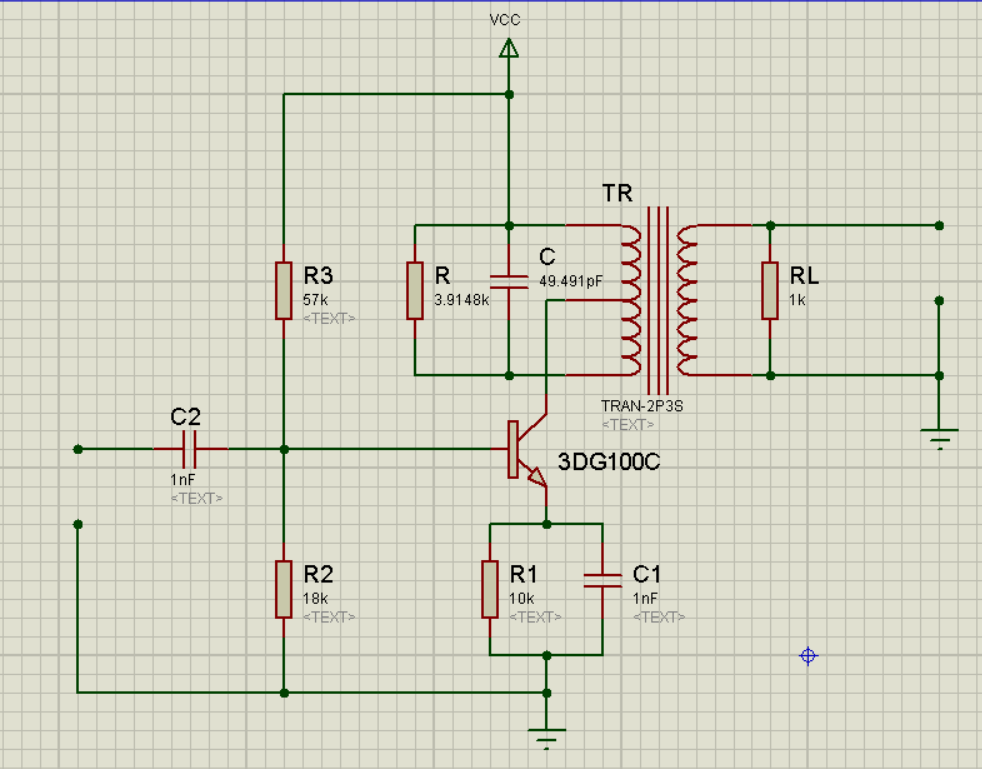
\includegraphics [width=0.75\textwidth]{figure//res.png}
	\caption{设计电路图}\label{remote1}
\end{figure}

\end{spacing}
\end{document}